\chapter*{Введение}

В работе рассматривается метод построения сценариев диалога на естественном языке с использованием условных планов в качестве модели. Актуальность темы обуславливается вектором развития программных продуктов в экосистеме наиболее известных операционных систем для мобильных устройств.

В апреле 2010 года Apple приобрела стартап ``Siri'' за \$250 млн. Основным приобретаемым продуктом было одноименное приложение -- персональный помощник и вопросно-ответная система. 4 октября 2011 года оно было представлено как часть программного обеспечения iPhone 4S. Принцип работы - голосовой диалог с пользователем, в ходе которого тот может получить информацию о погоде, котировках акций, новых сообщениях электронной почты, контролировать поведение устройства, включая воспроизведение музыки, создание событий в календаре и т.д.

\begin{wrapfigure}{r}{0.3\textwidth}
 \begin{center}
  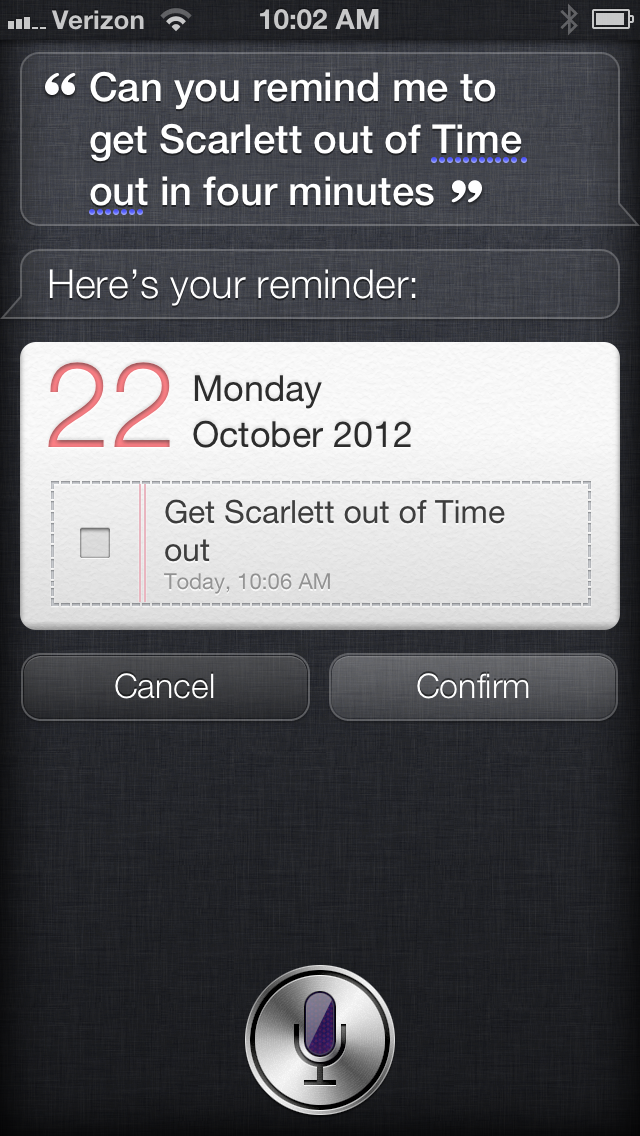
\includegraphics[height=5cm]{siri-timer}
  \caption{Приложение Siri}
 \end{center}
\end{wrapfigure}


Немногим позднее, в июне 2012 года, на очередной конференции Google I/O был представлен персональный помощник Google Now, имеющий сходную функциональность и поставляемый по умолчанию как часть операционной системы Android версии 4.1. Jelly Bean и выше.

Работа этих продуктов основывается на экспертных системах с базой знаний, а диалоговые возможности подкрепляются технологиями голосового поиска.

Другим примером является российская разработка ``Ассистент на русском'' компании i-Free. Это приложение для Android, по функционалу аналогичное описанным выше продуктам. Доступно открытое API для создания собственных модулей. Для распознавания контекста диалога используется сопоставление по базе шаблонов.

Анализ решений, рассмотренных выше, привел к пониманию, что для более естественного взаимодействия с пользователем необходимо:

\begin{itemize}
 \item Максимально полно использовать контекст предметной области диалога
 \item По возможности работать без постоянного подключения к сети Интернет.
\end{itemize}

В этой работе обсуждаются способы построения актуального контекста диалога, не зависящие от конкретной предметной области. В дальнейшем для реализации собственно диалогового модуля предполагается использовать доступные технологии распознавания голоса (Google Voice API) и подходы с использованием библиотек морфологии и синтаксического анализа русского языка (Yandex Tamitha), а также базу шаблонов, аналогичную той, что используется в приложении i-Free.

В первой главе излагаются основы теории интеллектуальных агентов и известные классические подходы к проблеме автоматического планирования в условиях полной наблюдаемости. Далее вводятся понятия для рассмотрения планирования в условиях частичной наблюдаемости на примере ``игрушечной'' проблемы планирования.

Вторая глава дает концептуальное описание построенного алгоритма планирования, затем детально разбираются использованные алгоритмы. Приводятся оценки сложности.

Третья глава посвящена программной реализации: выбору языковых средств, библиотек; общей архитектуре системы и взаимодействию ее компонентов. Дается описание внешних программных интерфейсов (API).

В четвертой главе приводятся примеры работы программы, пользовательского интерфейса и описание работы с помощью командной строки. Описываются подходы к тестированию созданного программного обеспечения.